\chapter[SIMULINK]{SISTEMA IMPLEMENTADO NO MATLAB\textsuperscript{TM} EM AMBIENTE SIMULINK} \label{sys:teo}

O sistema foi implementado no Matlab\textsuperscript{TM} usando os recursos \textit{Embedded} Matlab\textsuperscript{TM} \textit{Function Block}  (EMFB) do Simunlink. Nesta ferramenta pode-se descrever o \textit{encoder} e o \textit{decoder} da codificação 64b66b. Pela grande variedade de recursos que esta ferramenta possui é possível criar mecanismos para obter as características da codificação. Estas podem serem obtidas inserindo erros no dado transmitido do \textit{encoder} para o \textit{decoder} analisando o número de erros obtido pelo número de dados transmitidos. Estes erros inseridos devem ser aleatórios para a obtenção de uma característica que se aproxime da realidade.

A codificação 64b66b foi originalmente descrita para mapear os dados de 8 bits do protocolo XMGII, como descrito no capítulo \autoref{codificacao64b66b}. Este protocolo é responsável pela comunicação entre duas sistemas de hardwares diferentes no padrão ethernet 10GBASE-R IEEE 802.3: \textit{Media Access Control}(MAC) e o \textit{Physical Layer}(PHY). Portanto, a codificação possui uma parte de códigos para controle porém o objetivo do trabalho não necessita desta funcionalidade. O propósito do sistema é verificar se a codificação possui propriedades interessantes para ser implementada em um chip \textit{Field Programmable Gate Array }(FPGA). Desta forma, o único interesse é na transmissão de dados puros sendo desnecessário a descrição dos controles para o teste das propriedades da codificação. 

A codificação não possui uma característica robusta para detectar erros. Isto deve-se pelo fato do padrão ethernet ,para o qual foi designada, possuir um CRC-32 que gera bits redundantes, sendo estes adicionados no pacote da transmissão. Portanto, para este sistema inseriu-se um CRC 8 bit descrito na seção \autoref{crc8}. Um esquema do sistema implementado é representado na \autoref{esquema_64b66b}.

\begin{figure}[H]
	
	\caption{\label{esquema_64b66b} Esquema do sistema implementado da codificação 64b66b.}
	\centering
	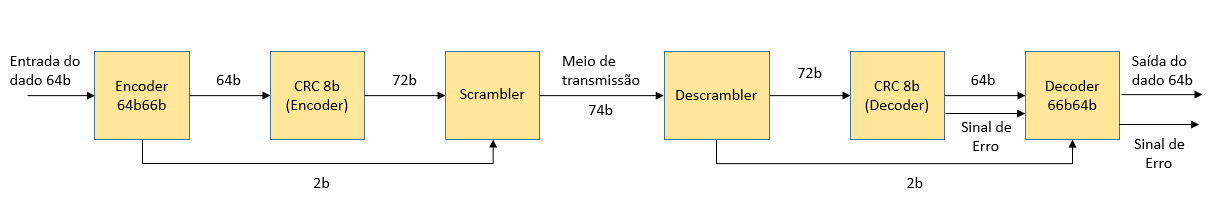
\includegraphics[scale=0.48]{esquema_codificacao64b66b.png}
	\begin{center}
		Fonte: Elaborado pelo Autor
	\end{center}	
\end{figure}


Na figura \autoref{sistema_64b66b} é ilustrado o sistema desenvolvido usando a ferramenta EMFB do Simulink. Neste sistema observa-se o bloco que possui a função $RandomBinary$ que realiza a inserção de dados binários randômicos de 64 bits. Os subsistemas $Bernoulli \quad Binary \quad Generator \quad (BBG)$ e $Aleatory \quad Counter \quad (ALC)$ são responsáveis por gerarem o erro na transmissão. Este erro é inserido após o codificador gerar um dado de 74 bits. 

No subsistema $Set \quad Error$ é aplicado o erro no dado transmitido e no subsistema Multiport Switch (MPS) é selecionado se há ou não erro na transmissão. No subsistema $Decoder \quad 66b \quad to \quad 64b \quad + \quad CRC \quad 8 \quad bits$  os dados são decodificados para 64 bits novamente. No subsistema $Display \quad Error$ o número de erros do sistema é obtido de quatro formas. Primeiramente analisa-se o sinal de saída do \textit{decoder} $Error\_out$,  caso estiver com valor lógico alto aciona um contador. A segunda obtêm-se o número de erros pela comparação entre os dados de entrada do \textit{encoder} com os dados de saída do \textit{decoder}, caso forem diferentes aciona um contador registrando o erro. A terceira é comparando o dado de 74 bits que entra no \textit{scrambler} com o dado de 74 bits de saída do \textit{descrambler}, o resultado é exibido na saída $ContErrorScrambler$ do bloco $Display \quad Error$. A quarta forma é a contagem de erros inseridos no canal, sendo exibido na saída $ContErrorInserted$ do bloco $Display \quad Error$  

\begin{figure}[H]
	\caption{\label{sistema_64b66b} Sistema da codificação 64b66b implementado no Matlab\textsuperscript{TM}(SIMULINK).}
	\centering
	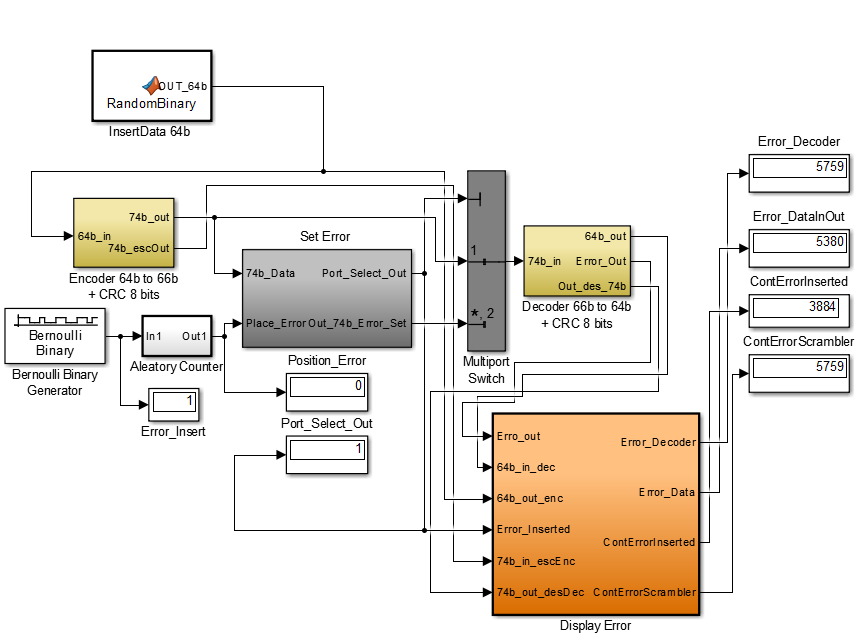
\includegraphics[scale=0.7]{sistema_64b66b.png}
	\begin{center}
		Fonte: Elaborado pelo Autor
	\end{center}	
\end{figure}

O subsistema BBG gera números binários de 1 bit (0’s ou 1’s) aleatoriamente de acordo com uma porcentagem pré-definida. Pode-se dizer que este subsistema é como se fosse uma moeda viciada, de acordo com um número total de eventos define-se a porcentagem do número de vezes que cada lado da moeda vai sair quando for jogada. O erro é gerado quando o subsistema gerar o bit 0, dessa forma dentro do subsistema pode-se definir a probabilidade de ocorrer erro no canal.

Na \autoref{aleatory_conter} observa-se a estrutura dentro do subsistema ALC que recebe o bit do BBG. Desta forma, caso o ALC receba um bit '0' do BBG é enviado um número aleatório ao subsistema $Set \quad Error$ representando a posição que o erro vai ser inserido no vetor de 74 bits. Caso o ALC receba um bit '0' do BBG então envia-se um número 0 para o $Set \quad Error$, não gerando nenhum erro na transmissão. O subsistema $Set \quad Error$ seleciona a porta 1 do MPS, se não for inserido erro, ou porta 2 quando não há erros na transmissão. Pela \autoref{aleatory_conter} observa-se a entrada In1 a qual recebe o bit do subsistema BBG selecionando,  através do bloco Switch, entre a constante de valor inteiro “1” ou o subsistema $Random \quad Integer \quad generator$ (RIG) adicionado com uma constante de valor inteiro “1” como saída.

O RIG está configurado para gerar números de “0” até “73”, dessa forma somado com a constante de valor inteiro “1” são gerados números de “1” até “73” aleatoriamente. O subsistema Switch seleciona a constante de valor 1 se na entrada In1 possuir o bit 1, caso possuir o bit 0 é selecionado o RIG adicionado com a constante 1. 

\begin{figure}[H]
	\caption{\label{aleatory_conter} Estrutura Interna do bloco Aleatory Counter.}
	\centering
	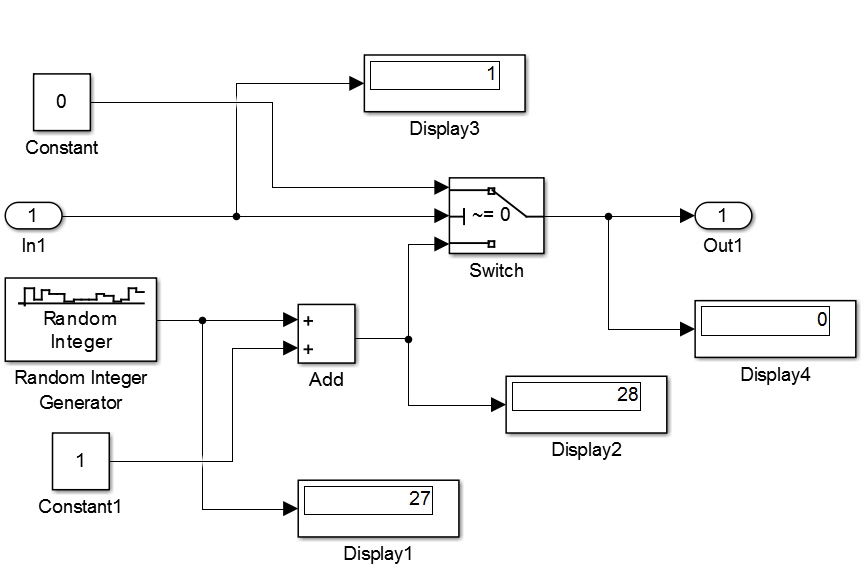
\includegraphics[scale=0.5]{aleatory_conter.png}
	\begin{center}
		Fonte: Elaborado pelo Autor
	\end{center}	
\end{figure}

No MPS a porta sem número é a que seleciona as portas 1 ou 2, dessa forma se na porta 1 é inserido o valor inteiro “1” logo é selecionado a porta $2$ e assim por diante. Pela \autoref{error_set}, no MPS o erro é inserido quando na porta 1 estiver presente o valor inteiro $2$. Dessa forma, pela lógica presente no subsistema ALC pode-se inserir um erro aleatoriamente no canal de transmissão. Na \autoref{error_set} apresenta-se a estrutura do subsistema Error Set que insere erros no dado de saída. No bloco está presente uma função que recebe uma posição para inserir o erro no dado transmitido. Caso esta posição seja diferente de 0, o erro é inserido no dado transmitido e a porta do MPS é selecionada para $2$. Caso o bit recebido seja $0$, é selecionado a posição 1 no MPS e nenhum erro é inserido.

\begin{figure}[H]
	\caption{\label{error_set} Estrutura interna do subsistema \textit{Set Error}.}
	\centering
	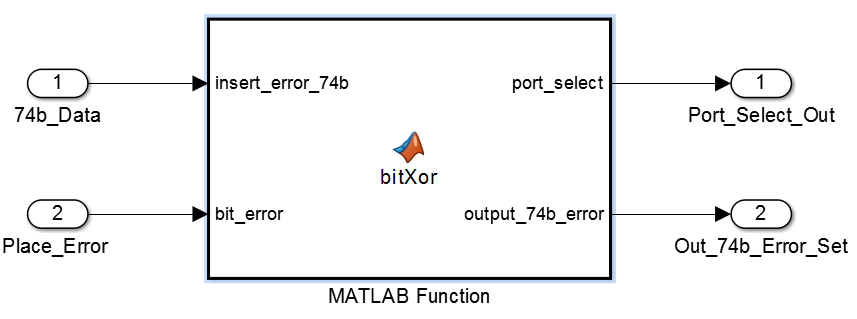
\includegraphics[scale=0.5]{error_set.png}
	\begin{center}
		Fonte: Elaborado pelo Autor
	\end{center}	
\end{figure}

Na \autoref{program_erroSet} é apresentado a programação do subsistema \textit{Matlab\textsuperscript{TM} Function} da \autoref{error_set} em que usa-se o comando \textit{bitxor} do Matlab\textsuperscript{TM} para realizar a operação XOR. Neste comando realiza uma operação XOR entre o dado transmitido de 74 bits e o um vetor de zeros de 74 bits setado o bit $1$ na posição de erro, definida no bloco ALC. 

\begin{figure}[H]
	\caption{\label{program_erroSet}  Programação interna do subsistema \textit{Matlab\textsuperscript{TM} Function}.} 
	\centering
	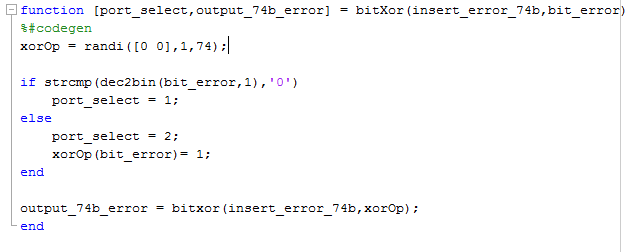
\includegraphics[scale=0.9]{program_errorSet.png}
	\begin{center}
		Fonte: Elaborado pelo Autor
	\end{center}	
\end{figure}

Na \autoref{enc_64b66b} é apresentado a estrutura interna do subsistema \textit{Encoder} 64b to 66b. Nesta estrutura está presente um \textit{Function Block} em que está descrito a codificação do \textit{encoder} 64 bits para 66 bits. Como está presente o CRC 8 bits nesta estrutura, o dado de saída possui 74 bits. A programação completa do \textit{Function Block Encoder 64b66b} está descrita no \autoref{enc:64b}.

\begin{figure}[H]
	\caption{\label{enc_64b66b}  Estrutura interna do Encoder 64b to 66b.}
	\centering
	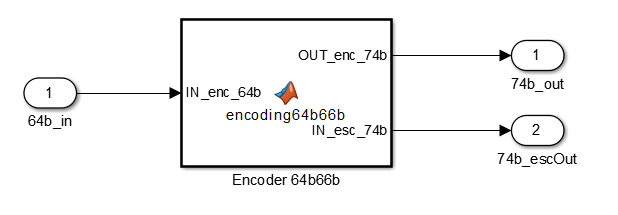
\includegraphics[scale=0.7]{enc_64b66.png}
	\begin{center}
		Fonte: Elaborado pelo Autor
	\end{center}	
\end{figure}

Na \autoref{dec_66b64b} é apresentado a estrutura interna do subsistema \textit{Decoder} 64b to 66b. Nesta estrutura está presente um \textit{Function Block} em que está descrito a codificação do \textit{Decoder} 66 bits para 64 bits. Como possui um CRC 8 bits implementado o dado recebido é de 74 bits. A programação completa do \textit{Function Block Decoder} 66b64b está descrita no \autoref{dec:64b}.

\begin{figure}[H]
	\caption{\label{dec_66b64b}  Estrutura interna do \textit{Decoder} 66b to 64b.}
	\centering
	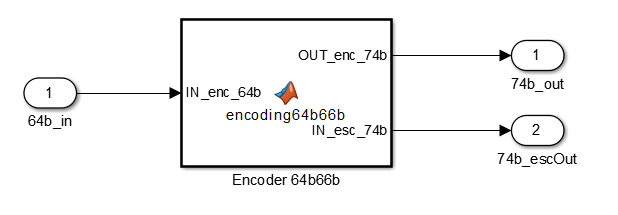
\includegraphics[scale=0.7]{enc_64b66.png}
	\begin{center}
		Fonte: Elaborado pelo Autor
	\end{center}	
\end{figure}

Na \autoref{display_error} é apresentado a estrutura interna do subsistema \textit{Display Error}. A estrutura possui 6 entradas sendo a primeira o sinal de saída $Error\_Out$ do \textit{Decoder}, indicando um sinal de erro do dado recebido. O par de entrada $64b\_in\_dec$ e $64b\_out\_enc$ representam o dado de 64b de saída do \textit{decoder} e entrada do \textit{encoder}, respectivamente. O outro par de entrada $74b\_in\_escEnc$ e $74b\_out\_desDec$, representam o dado de 74 bits que entra no \textit{escrambler} e o que sai do \textit{descrambler}, respectivamente. A entrada $Error\_Inserted$ é a porta que foi selecionado no MPS, desta forma quando é recebido o valor 2 um contador é acionado na função $errorContPort$ sendo possível obter o número de erros do sistema.

\begin{figure}[H]
	\caption{\label{display_error}  Estrutura interna do subsistema \textit{Display Error}.}
	\centering
	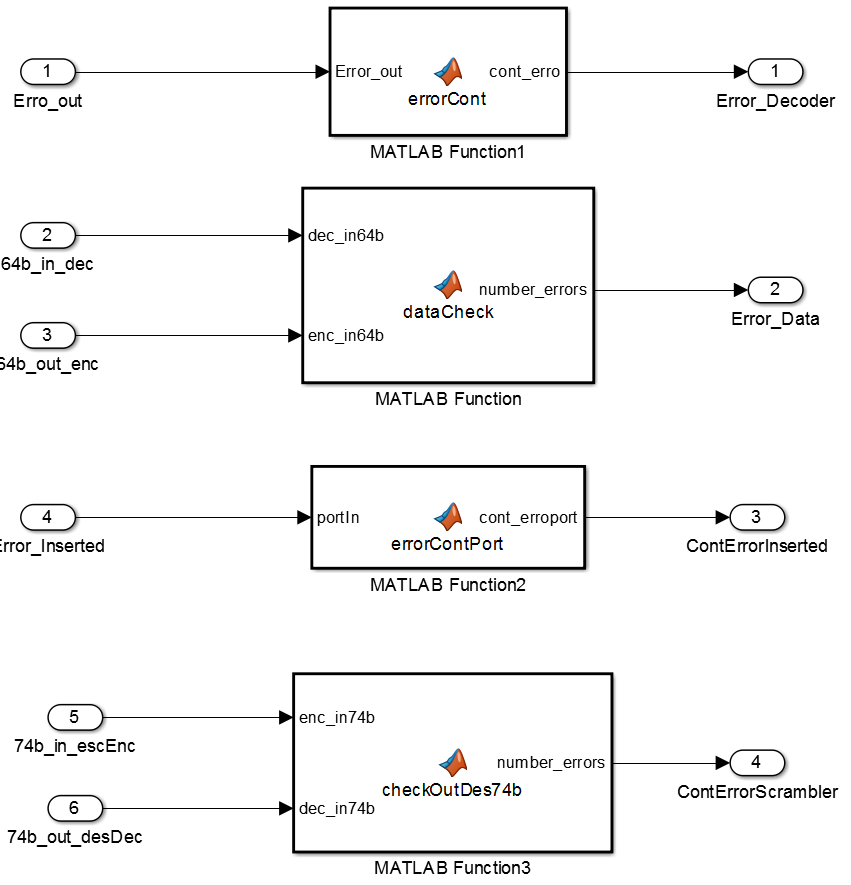
\includegraphics[scale=0.5]{display_error.png}
	\begin{center}
		Fonte: Elaborado pelo Autor
	\end{center}	
\end{figure}


Todos os códigos das funções implementadas no sistema estão descritos nos apêndices no final do trabalho.


